\chapter{Cryptocurrencies}
\label{Cryptocurrencies}

There were hundreds of failed attempts of creating cryptographic payment systems before cryptocurrencies like Bitcoin and Ethereum came into existence. Some of these systems are listed in Figure \ref{paymentSystems}. All of them were created before Bitcoin. Despite that, only a few of them survived to these days. Some of these attempts were only academic proposals while others were deployed and tested systems. One of the survival is PayPal. It is only because it quickly gave up its original idea of hand-held devices for cryptographic payments. \cite{wayner1997digital}

So there is a question, what makes cryptocurrencies successful nowadays?  It may be easy to use principle and no need for external hardware. 
Another critical component of cryptocurrencies discussed in this work is blockchain. Generally, it is a ledger in which all transactions are securely stored. The idea behind blockchains is pretty old, and it was initially used for timestamping digital documents. \cite{haber1990time} 


\begin{figure}[h]
    \centering
    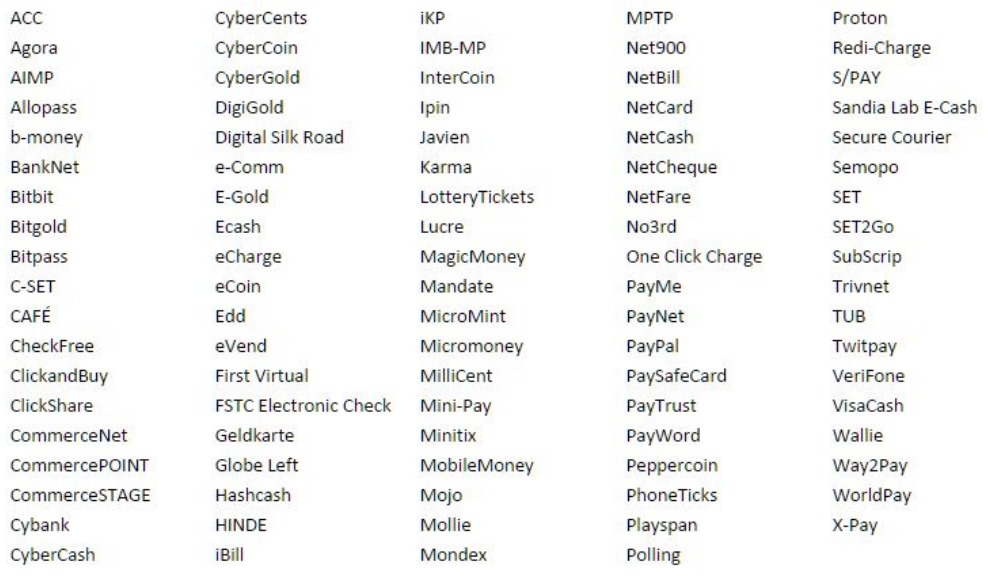
\includegraphics[width=14cm]{failedCryptos.PNG}
    \caption{Electronic payment systems before cryptocurrencies \cite{narayanan2016bitcoin}}
    \label{paymentSystems}
\end{figure}


\section{Bitcoin}
Bitcoin is probably the most famous cryptocurrency. It started as a digital currency transaction protocol but founded a new concept of blockchain \cite{ChowdhuryNiaz2020Ibba}. On 3\textsuperscript{rd} January 2009, Satoshi Nakamoto (an alias for a person or group persons authored the bitcoin white paper) mined the genesis block of bitcoin (block with height 0). Satoshi got the reward of 50 bitcoins (half a million US dollars in the time of writing). This text was embedded in the genesis\footnote{\url{https://en.bitcoin.it/wiki/Genesis\_block}} block (see Figure \ref{genesisBitcoin}): \textit{The Times 03/Jan/2009 Chancellor on brink of second bailout for banks} \cite{newYorkerBTC}. Bitcoin has a limited supply of coins to approximately 21 million. New coins are emitted only when a new block is created \cite{nakamoto2008peer}.

\begin{figure}[h]
    \centering
    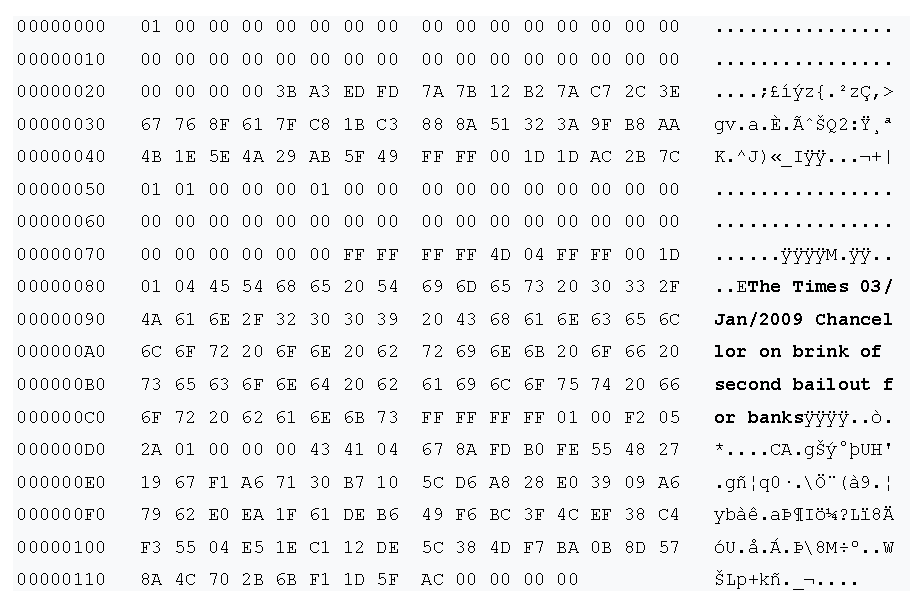
\includegraphics[width=14cm]{genesisBitcoin.pdf}
    \caption{Genesis bitcoin block}
    \label{genesisBitcoin}
\end{figure}

First documents purchase happened in 22\textsuperscript{nd} May 2010, when Laszlo Hanyecz bought two pizzas for 10,000 bitcoins (\$41 then, now about \$80,000 000)\footnote{\url{https://bitcointalk.org/index.php?topic=137.0}}. This transaction hash is \texttt{a1075db55d416d3ca199f55b6084e\-2115b9345e16c5cf302fc80e9d5fbf5d48d} and is stored in bitcoin blockchain forever\footnote{Actual photos of \$80,000,000 pizza are on \url{http://heliacal.net/~solar/bitcoin/pizza/}}.


\section{DigiByte}
DigiByte was developed and released in 2013. It is based on Bitcoin with some adjustment in the code to improving functionality. In late 2017 there was 200,000 pending transaction in Bitcoin. Miners preferred transaction with a higher fee, so to confirm a transaction, user needed to pay \$50. DigiByte solved this problem by adding a new block every 15 seconds (new block in Bitcoin is mined every 10 minutes). Average transaction occupies 570 bytes of data. One block can contain approximately 3,500 transactions given the 2 MB limit. This restriction means that in DigiByte, 230 transactions can be confirmed in one second compared to Bitcoin 4-7 transaction per second. DigiByte also has 1,000:1 DigiByte to Bitcoin ratio, so for every Bitcoin, there is 1,000 DigiByte. \cite{digibyteBook}


\section{Ethereum}
Ethereum, rather than a cryptocurrency, is a blockchain application platform with Turing-complete programming language. While both the Bitcoin and Ethereum networks are powered by the principle of distributed ledgers and cryptography, the two differ technically in many ways. For example, transactions on the Ethereum network may contain executable code, while data affixed to Bitcoin network transactions are generally only for keeping notes. Other differences include block time (an ether transaction is confirmed in seconds compared to minutes for bitcoin) and the algorithms that they run on (Ethereum uses ethash while Bitcoin uses SHA-256). \cite{wood2014ethereum, buterin2014next}



\section{Decred}
Decred is cryptocurrency build from Bitcoin. The main difference from Bitcoin is the rewarding system from mining. In Bitcoin, the miner gets full reward for a mined block. Sometimes, the Bitcoin blockchain splits when two or more miners found a block at nearly the same time. The fork is resolved when the subsequent block(s) are added, and one of the chains becomes longer than the alternative(s). In Decred the chance of blockchain forks is minimized by hybrid proof of work and proof of state system. Each time a block is created (by a miner), it is not automatically part of the blockchain. Block needs to be approved by ticket holders. Then miner receives a block reward (newly created DCR). If the block is rejected by ticket holders, the miner does not receive a reward. Tickets holders for a new block are chosen randomly. The ticket validates the previous block. A~block needs at least three of the five votes chosen to approve it for it to be validated.  This hybrid system has many implications, including making a 51\% power attack very difficult and making a minority fork very difficult as well. \cite{decredWhitePaper}

\section{Monero}
Three years after Bitcoin, in 2012, the competing Bytecoin cryptocurrency entered the market. The problem with this cryptocurrency, however, was that 80\% of all coins were mined in advance by its authors. The chances of mining were, therefore, not balanced. This injustice led to the decision that this cryptocurrency would start again. New cryptocurrency starts on 18 April 2014 and was called BitMonero, a composite of the word coin in Esperanto (Monero) and Bitcoin according to Bitcoin. However, after five days, the community decided to use only Monero for short. Monero's significant advantage is the dynamic size of the mined blocks. Bitcoin has one block size limited to 1 MB, while Monero adapts the block size to the network load. If the number of transactions increases, so does the block size to accommodate all transactions. Thus, unlike Bitcoin, the more transactions users make, the lower the transaction fee. Monero's main benefit is its full anonymity and interchangeability thanks to CryptoNote protocol \cite{van2013cryptonote}. Monero hides recipient and sender addresses. \cite{moneroTracebility}

\section{Analysis of Current Blockchain Explorers}
A~Blockchain Explorer is a web application that allows us to explore the whole blockchain. Their primary function is to allow everyone with an Internet connection to track in real-time all the transactions or interactions made by each cryptocurrencies holders, regardless of his or her level of knowledge and expertise. \cite{laurence2019blockchain, dhillon2017blockchain}


\subsection{Blockbook}
As a representative of traditional explorers, we chose Blockbook. Blockbook\footnote{\url{https://github.com/trezor/blockbook}} is a blockchain indexer for Trezor Wallet\footnote{\url{https://wallet.trezor.io/}}, developed by SatoshiLabs\footnote{\url{https://satoshilabs.com/}}. It currently supports more than 30 coins (and the community implemented some others). For data storage, Blockbook is using RocksDB\footnote{\url{https://github.com/facebook/rocksdb/wiki}} developed by Facebook, which is a NoSQL database that stores only key-value pairs. Blockbook is providing fast API for accessing blocks, addresses and transactions. Main limitations of Blockbook are:
\begin{itemize}
    \item \textbf{Not distributed} (client-server architecture) -- problem with scaling for more users. 
    \item \textbf{Not an SQL database} -- it does not have a relational data model, it does not support SQL queries, and it has no support for indexes.
    \item \textbf{Single-Process} -- only a single process (possibly multi-threaded) can access a particular database at a time.
\end{itemize}
